\section{Evaluation}

We evaluated Syndicate using microbenchmarks to test local write performance, metadata read-write
 performance, and remote sequential read performance.  In the last experiment, 
we make use of two different CDNs to drive data distribution:  Verivue Hypercache~\cite{vcoblitz}
 and CoBlitz~\cite{CoBlitz}.  Verivue Hypercache is an industrial implementation 
of CoBlitz which we deployed in VICCI to create a private CDN for Syndicate clients only.  
We use the publicly-accessible deployments of CoBlitz as well as the Verivue 
Hypercache to characterize Syndicate's read performance independently of the CDN deployment
and workload.

In order for Syndicate to scalably deliver data to its clients, it must
not impose additional performance bottlenecks on the CDN.  Our experiments are 
designed to examine the performance of Syndicate itself, as opposed to
the underlying CDN, to determine whether or not our prototype meets this requirement.

\subsection{Local Writes}

To test Syndicate's local write performance, we used the FileBench filesystem benchmarking 
tool~\cite{filebench} to create 50,000 files representing 778.397MB of file data in a Syndicate client.
We measured the average number of I/O operations per second, the average write throughput, and the average
operation latency.  The files were generated with the \texttt{createfiles} benchmark. 
Our tests employed a single writer to simulate the act of a user generating a filesystem tree
to publish via Syndicate.  Our benchmark ran on a Dell PowerEdge R410 server running
CentOS 5.7 (Linux 2.6.18) with an Intel Xeon X5650, 48GB of RAM, and three 1TB disks logically 
managed as a single disk.

\begin{figure}[h!]
\centering
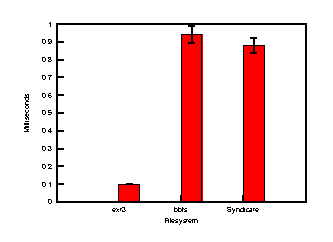
\includegraphics[width=0.5\textwidth]{data/low-latency/latency}
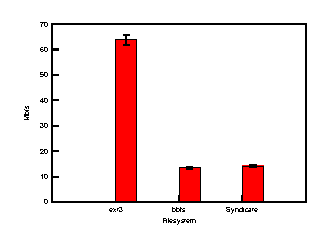
\includegraphics[width=0.5\textwidth]{data/low-latency/write}
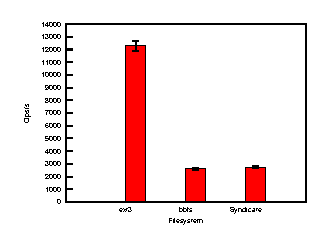
\includegraphics[width=0.5\textwidth]{data/low-latency/ops}
\caption{Average filesystem I/O latencies, write bandwidths, and operations per second.  The error bars represent one standard deviation.}
\label{fig:low-latency}
\end{figure}

We compared Syndicate's local write performance to the ext3 filesystem on our server and a simple FUSE filesystem
called Big Brother FS (BBFS)~\cite{fuse-tutorial} in Figure~\ref{fig:low-latency}.
BBFS simply redirects any requested filesystem operations to an underlying directory and 
logs the operation, and does as little data processing as possible beyond this.  As such, we believe
that it is suitable to compare Syndicate to BBFS in this experiment to determine how the additional
processing Syndicate performs on its write requests affects its overall write performance.

We ran the FileBench \texttt{createfiles} benchmark five times on each filesystem.
BBFS and Syndicate achieve comparable performance, but surprisingly Syndicate is slightly
faster than BBFS.  This is because Syndicate, unlike BBFS, uses the direct I/O feature in FUSE, which allows it
to process larger amounts of data at once at the expense of additional code complexity.
This more than makes up for the additional processing it must perform relative to BBFS.

Not surprisingly, both FUSE filesystems performed considerably worse than ext3 because
they run in userspace and redirect file I/O operations to underlying storage.
However, the performance is not unacceptably slow--Syndicate achieves $14.14$ Mbps 
throughput and $2726$ operations per second, with an average operation latency of $0.88$ milliseconds.

\subsection{Metadata Reads and Writes}

We evaluated the Syndicate metadata server's write performance without network constraints
by running a metadata server locally with a client.  We created filesystem hierarchies of 
$1000$, $5000$, $100000$, and $50000$ files using the FileBench tool's \texttt{createfiles} 
benchmark (with otherwise default settings) within a local Syndicate client connected to the
metadata server, and configured the client to wait until the \texttt{createfiles} execution 
was done to upload all of the resulting metadata.  We then measured how long it took the metadata
server to process the list of metadata updates.  Once the metadata server had added
each metadata update to its master copy, we started a fresh client and measured how long it
took the client to download and recreate the hierarchy in its mountpoint.

\begin{figure}[h!]
\centering
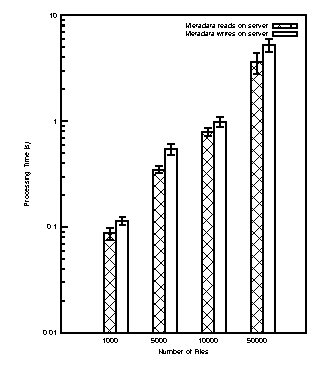
\includegraphics[width=0.5\textwidth]{data/metadata/metadata}
\caption{Total time taken to read and write metadata by the client and metadata server,
respectively.  The Y axis is on a logarithmic scale.  The error bars are one standard
deviation.}
\label{fig:metadata-io}
\end{figure}

\begin{table*}[ht!]
\begin{tabular}{ | l | l | l | l | }
\hline
\textbf{Hierarchy Size} & \textbf{Read (client)} & \textbf{Write (metadata server)} \\
\textbf{1000 files} & $0.08732\pm0.0111s$ & $0.1140\pm0.00952s$ \\
\textbf{5000 files} & $0.34819\pm0.0274s$ & $0.5400\pm0.06210s$ \\
\textbf{10000 files} & $0.78944\pm0.0713s$ & $0.9902\pm0.10146s$ \\
\textbf{50000 files} & $3.59741\pm0.80014s$ & $5.2003\pm0.74801s$ \\
\hline
\end{tabular}
\caption{Average times ($\pm$ standard deviation) over five runs required for a client to process a hierarchy
of the given size, and the average times over five runs required for a metadata server to process the same hierarchy.}
\label{tab:metadata-io-table}
\end{table*}

The results of our metadata read and write performance experiment are summarized in Figure~\ref{fig:metadata-io} and Table~\ref{tab:metadata-io-table}.
We ran our experiment on a Lenovo Thinkpad T510 with an Intel Core i7-620M CPU and 4GB RAM.  We calculated the
read and write performance on each hierarchy five times.  Our plot shows error bars of one standard deviation.
It only took the metadata server an average of $5.2s$ to process a $50000$-file hierarchy, and it only
took the Syndicate client an average of $3.6s$ to recreate the same hierarchy by iteratively requesting
directories from the metadata server for which it did not have up-to-date information.

\subsection{Sequential Reads}

We tested Syndicate's remote read performance by copying files of various sizes out of
a mounted Syndicate filesystem.  We compared a single host's read performance when it 
downloaded the file data directly from its origin to its performance when it downloaded
the data from a CDN.  The data was hosted on a VICCI sliver in Washington University, 
and the client downloading it ran on a laptop in Princeton.  The Verivue Hypercache
directed our requests to nodes running on VICCI slivers in Georgia Tech.  We warmed
the caches in both CoBlitz and Hypercache by requesting the file twice with 
the \texttt{wget} command before running our experiment with Syndicate, to verify
that the data was pulled into the caches.

\begin{figure}[h!]
\centering
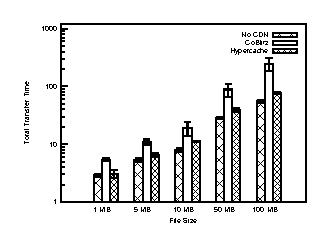
\includegraphics[width=0.5\textwidth]{data/sequential-read/sequential-read}
\caption{Total download times of datasets of various sizes in which Syndicate used CoBlitz, Hypercache, 
or a direct connection to the origin host to stream content.  The Y axis is on a logarithmic
scale.  The error bars are one standard deviation.}
\label{fig:sequential-read}
\end{figure}

\begin{table*}[ht!]
\begin{tabular}{ | l | l | l | l | l | l | }
\hline
 & \textbf{1 MB} & \textbf{5 MB} & \textbf{10 MB} & \textbf{50 MB} & \textbf{100 MB} \\
\textbf{No CDN} & $2.888\pm0.164s$ & $5.389\pm0.491s$ & $7.87\pm0.586s$ & $28.675\pm0.870s$ & $55.182\pm2.641s$ \\
\textbf{CoBlitz} & $5.392\pm0.364s$ & $10.966\pm1.086s$ & $18.990\pm5.104s$ & $88.364\pm22.704s$ & $248.624\pm62.563s$ \\
\textbf{Hypercache} & $3.075\pm0.465s$ & $6.516\pm0.543s$ & $11.247\pm0.186s$ & $39.238\pm3.75s$ & $77.538\pm2.977s$ \\
\hline
\end{tabular}
\caption{Average download time $\pm$ standard deviation of files of given sizes, achieved by Syndicate downloading
directly from the remote host or from either CoBlitz or Hypercache.}
\label{tab:sequential-read-table}
\end{table*}


We used the UNIX \texttt{cp} command to copy data from a mounted Syndicate filesystem
to local storage, which requests data in 32,768 byte chunks.  We plotted the average time
taken by the \texttt{cp} command on a logarithmic scale in Figure~\ref{fig:sequential-read}.
The raw data can be seen in Table~\ref{tab:sequential-read-table}.  We copied each file
into local storage five times, and measured the average time and standard deviation of our samples.
As desired, the read times are proportional to the size of the file.

We notice that Syndicate achieved the best read performance when reading directly from
a remote client.  This should not be misinterpreted the best course of action, since
there was only one reader in this experiment.  It is well known~\cite{slashdot-effect}
that many concurrent readers can overwhelm an origin server.  Both CDNs took longer
to deliver the data to Syndicate because both CDN implementations incur an overhead
processing cost for each fixed-size chunk of data served.  CoBlitz and Hypercache break
client requests into requests for fixed-sized byte ranges to the origin server, and cache
and reassemble the chunks on a client's behalf.  CoBlitz achieved less consistent and slower
performance because it is a publicly-useable CDN, and caches data for many other clients
besides Syndicate~\cite{codeen}.


\comment{

% this belongs here, but perhaps in less detail	
\subsection{CDN}

We use CoBlitz as the underlying CDN~\cite{coblitz}. CoBlitz
automatically redirects a user's HTTP GET request for content to the
best cache node that can service it.  This satisfies our first
assumption that cached data are uniquely identified by a single URL.
Also, if the HTTP GET request has a no-cache header~\cite{HTTP-RFC},
CoBlitz does not return cached data, satisfying our third assumption.

A web URL can be transformed into a CoBlitz-specific URL by appending the URL to a CDN prefix--a fully-qualified hostname that resolves to CoBlitz's request redirection nodes.  For example, if the CDN prefix is \texttt{http://coblitz.foo.com}, and a client must read a file whose URL is \texttt{http://www.bar.org/baz.dat}, the client must request the data from \texttt{http://coblitz.foo.com/www.bar.org/baz.dat}.  This satisfies our second assumption about the underlying CDN.

CoBlitz is highly fault-tolerant and easily configured, and demonstrates
excellent aggregate read throughput~\cite{codeen}.  CoBlitz breaks a
request for a file into requests for fixed-length chunks of the file,
which it then spreads across nodes using a consistent hashing scheme.
A node fetches and reassembles the chunks into a whole file to serve
to a client.  Node failures are handled transparently and are
invisible to the client. Nodes are centrally managed by a content
management interface, which exposes a ``purge content''
feature that our metadata server is able to leverage.

}

